\documentclass[journal,12pt,onecolumn]{IEEEtran}
\usepackage{mathtools,amssymb,amsfonts}
\usepackage{algorithmic}
\usepackage{algorithm}
\usepackage{graphicx}
\usepackage{xcolor}
\usepackage{float}
\usepackage{setspace}
\usepackage{subcaption}
\usepackage[hidelinks]{hyperref}
\usepackage{multirow}

% Double spacing
\doublespacing

\hypersetup{
   colorlinks=true,
   linkcolor=blue,
   citecolor=black,
   urlcolor=blue
}

% Improve section spacing
\usepackage{titlesec}
\titlespacing*{\section}{0pt}{12pt plus 4pt minus 2pt}{12pt plus 2pt minus 2pt}
\titlespacing*{\subsection}{0pt}{12pt plus 4pt minus 2pt}{8pt plus 2pt minus 2pt}
\titlespacing*{\subsubsection}{0pt}{12pt plus 4pt minus 2pt}{6pt plus 2pt minus 2pt}

\title{Genetic Algorithms: De Jong Test Functions}
\author{
   \IEEEauthorblockN{Matthew D. Branson} \\
   \IEEEauthorblockA{\textit{Department of Computer Science} \\
   \textit{Missouri State University}\\
   Springfield, MO \\
   branson773@live.missouristate.edu
   }
}

\date{June 24, 2025}

\begin{document}

\maketitle

\begin{abstract}
This paper presents the implementation and analysis of a binary-encoded genetic algorithm (GA) for optimizing four De Jong test functions: Sphere, Weighted Sphere, Step, and Noisy Quartic. The GA employs fitness-proportionate selection, two-point crossover, and bitwise mutation to evolve populations of 20 individuals over 50 generations. Experiments compare 8-bit and 16-bit encodings to evaluate the impact of precision on optimization performance. Results demonstrate successful convergence to near-optimal solutions for all functions, with 16-bit encoding achieving superior results for continuous functions. The Sphere function exhibited the fastest convergence due to its smooth landscape, while the Weighted Sphere proved most challenging due to its narrow valley structure. The Step function's discrete nature and the Noisy Quartic's stochastic evaluation highlight the GA's robustness in handling diverse optimization challenges where traditional methods may fail.
\end{abstract}

\begin{IEEEkeywords}
Genetic Algorithms, Binary Encoding, De Jong Test Functions, Optimization, Evolutionary Computing, Metaheuristics
\end{IEEEkeywords}

\section{Q1: Binary Encoding and Initialization}

\subsection{Variable Encoding}
Binary encoding was implemented for each continuous variable using both 8-bit and 16-bit representations. For a variable $x_i$ with bounds $[L_i, U_i]$, the encoding precision is:
\begin{equation}
\epsilon = \frac{U_i - L_i}{2^n - 1}
\end{equation}
where $n$ is the number of bits. For example, the Sphere function with range $[-5.12, 5.12]$ achieves precision $\epsilon = 0.0401$ with 8-bit encoding and $\epsilon = 0.000156$ with 16-bit encoding.

\subsection{Generating Initial Population}
The \texttt{generate\_population()} method creates random binary chromosomes by generating random bits (0 or 1) for each position. For a problem with $k$ variables encoded with $n$ bits each, the chromosome length is $k \times n$. A population of 20 individuals is initialized, with each chromosome representing a potential solution in the search space.

\section{Q2: Chromosome Decoding and Function Evaluation}

\subsection{Decoding a Chromosome}
Binary chromosomes are decoded to real values using linear mapping. For each variable, the binary substring is first converted to decimal, then mapped to the function domain:
\begin{equation}
x_i = L_i + \frac{U_i - L_i}{2^n - 1} \times \text{decimal}(b_i)
\end{equation}
where $b_i$ is the binary substring for variable $i$. This ensures uniform distribution across the search space.

\subsection{Function Evaluation}
Four De Jong test functions were implemented:
\begin{itemize}
    \item \textbf{f1 - Sphere}: $f(\mathbf{x}) = \sum_{i=1}^{3} x_i^2$, minimum at origin
    \item \textbf{f2 - Weighted Sphere}: $f(x_1,x_2) = 100(x_1^2 - x_2)^2 + (1 - x_1)^2$, minimum at $(1,1)$
    \item \textbf{f3 - Step}: $f(\mathbf{x}) = \sum_{i=1}^{4} \lfloor x_i \rfloor$, minimum at boundary
    \item \textbf{f4 - Noisy Quartic}: $f(\mathbf{x}) = \sum_{i=1}^{4} i \cdot x_i^4 + \text{random}[0,1)$, minimum near origin
\end{itemize}
Each function presents unique optimization challenges: f1 is smooth and unimodal, f2 has a narrow valley, f3 is discontinuous, and f4 includes stochastic noise.

\section{Q3: Genetic Algorithm Operations}

\subsection{Fitness Proportionate Selection}
Roulette wheel selection was implemented for minimization problems. Fitness values are transformed using $f'_i = 1/(f_i + 1)$ to favor lower values. For functions with negative fitness (e.g., Step function), values are first shifted to ensure positivity. Selection probability for individual $i$ is:
\begin{equation}
p_i = \frac{f'_i}{\sum_{j=1}^{N} f'_j}
\end{equation}
Individuals are selected by generating a random number and finding the corresponding cumulative probability interval.

\subsection{Crossover}
Two-point crossover was implemented with probability $p_c = 0.90$. Two random points $c_1$ and $c_2$ are selected where $1 \leq c_1 < c_2 < L$, and the genetic material between these points is exchanged:
\begin{align}
\text{Offspring}_1 &= P_1[1:c_1] + P_2[c_1:c_2] + P_1[c_2:L] \\
\text{Offspring}_2 &= P_2[1:c_1] + P_1[c_1:c_2] + P_2[c_2:L]
\end{align}
This operator promotes exploration while preserving building blocks.

\subsection{Bitwise Mutation}
Mutation is applied with probability $p_m = 1/L$ per bit, where $L$ is chromosome length. Each bit has an independent chance of flipping from 0 to 1 or vice versa. This low mutation rate maintains population diversity while preventing disruption of good solutions.

\section{Q4: Genetic Algorithm Execution}

\subsection{Execution of the Genetic Algorithm}
The genetic algorithm was executed with a population size of 20 individuals for 50 generations across all four De Jong test functions. Each run utilized both 8-bit and 16-bit binary encodings to investigate the impact of precision on optimization performance. The GA employed fitness-proportionate selection (roulette wheel), two-point crossover with probability 0.90, and bitwise mutation with probability $1/L$ where $L$ is the chromosome length.

\subsection{Fitness Evaluation}
Figures~\ref{fig:f1} through \ref{fig:f4} show the evolution of best and average fitness values across generations for each function.

\begin{figure}[H]
\centering
\begin{subfigure}{0.48\textwidth}
    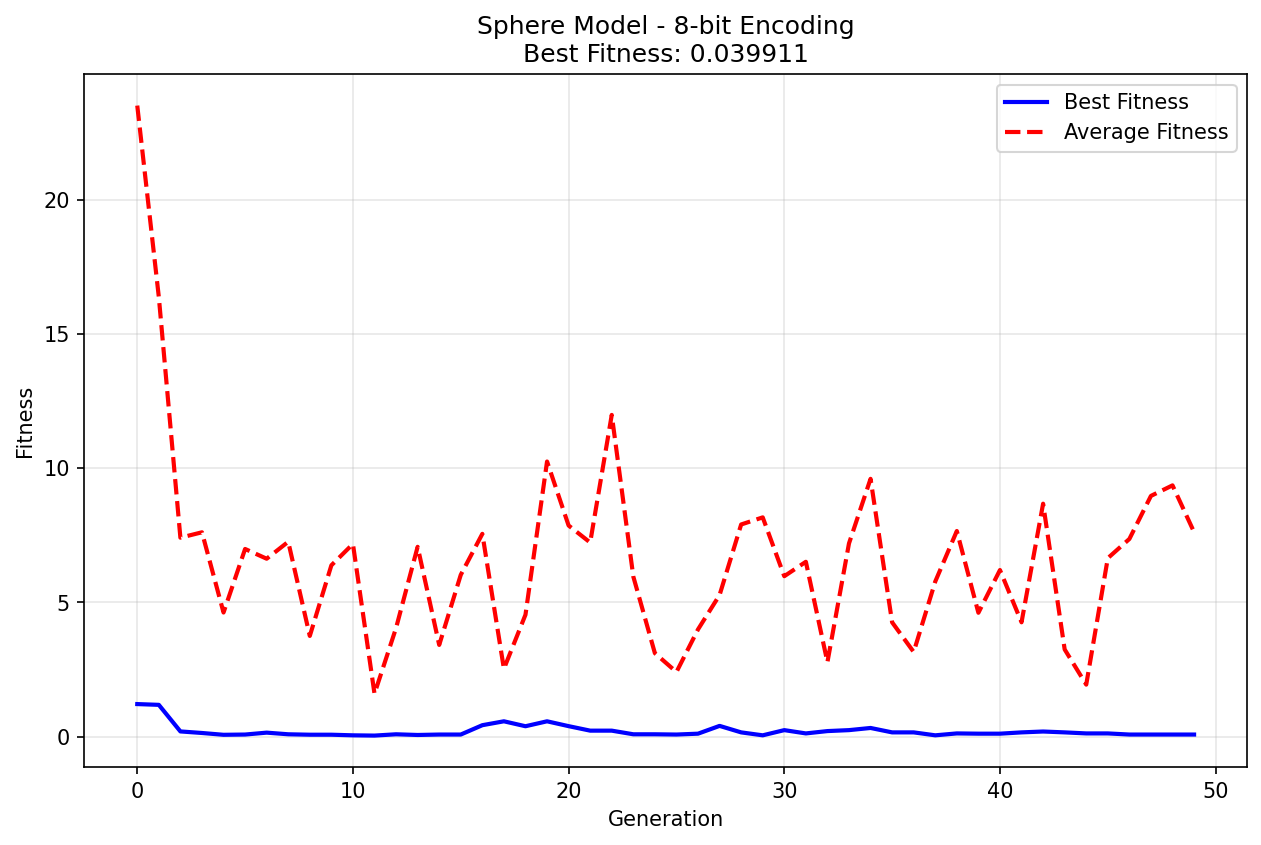
\includegraphics[width=\textwidth]{f1_8bit_fitness.png}
    \caption{8-bit encoding}
\end{subfigure}
\begin{subfigure}{0.48\textwidth}
    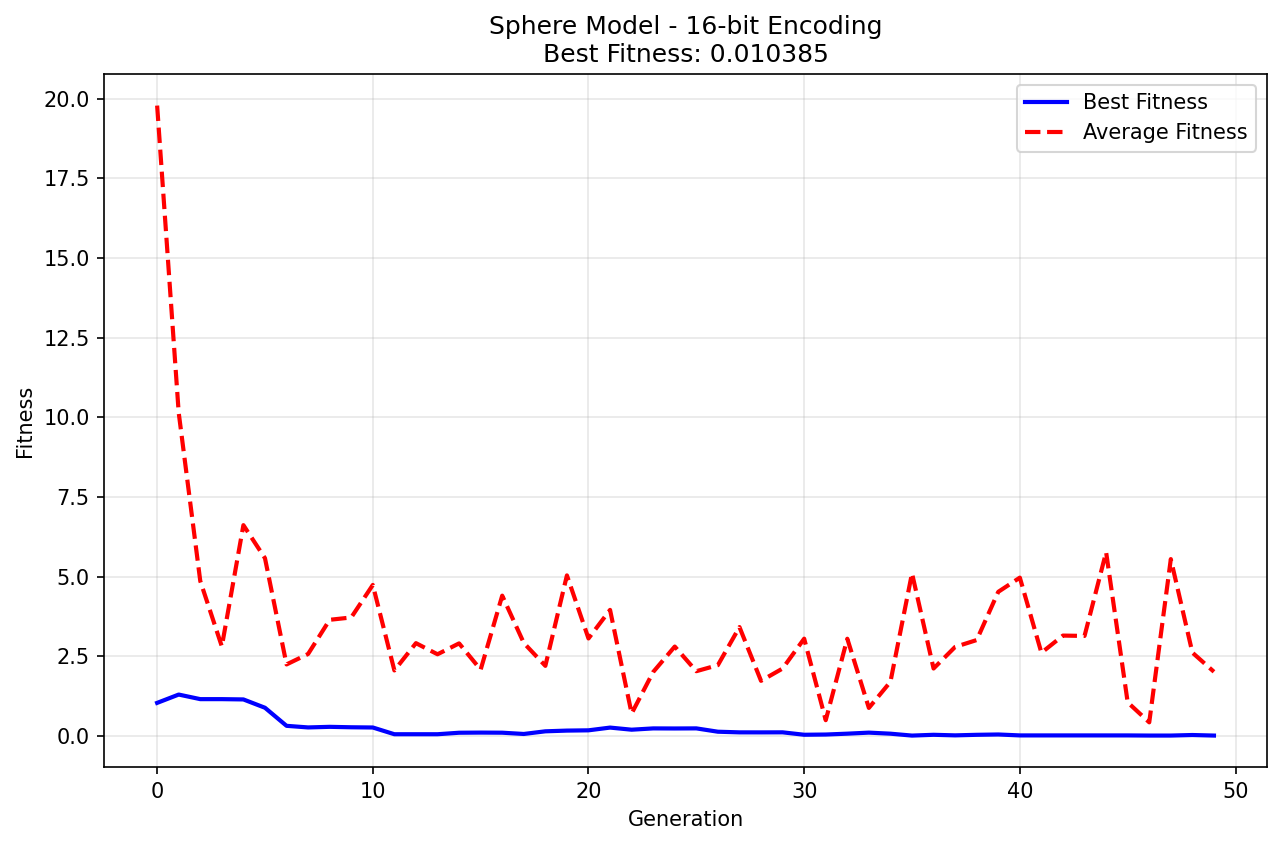
\includegraphics[width=\textwidth]{f1_16bit_fitness.png}
    \caption{16-bit encoding}
\end{subfigure}
\caption{Sphere Model (f1) convergence behavior}
\label{fig:f1}
\end{figure}

\begin{figure}[H]
\centering
\begin{subfigure}{0.48\textwidth}
    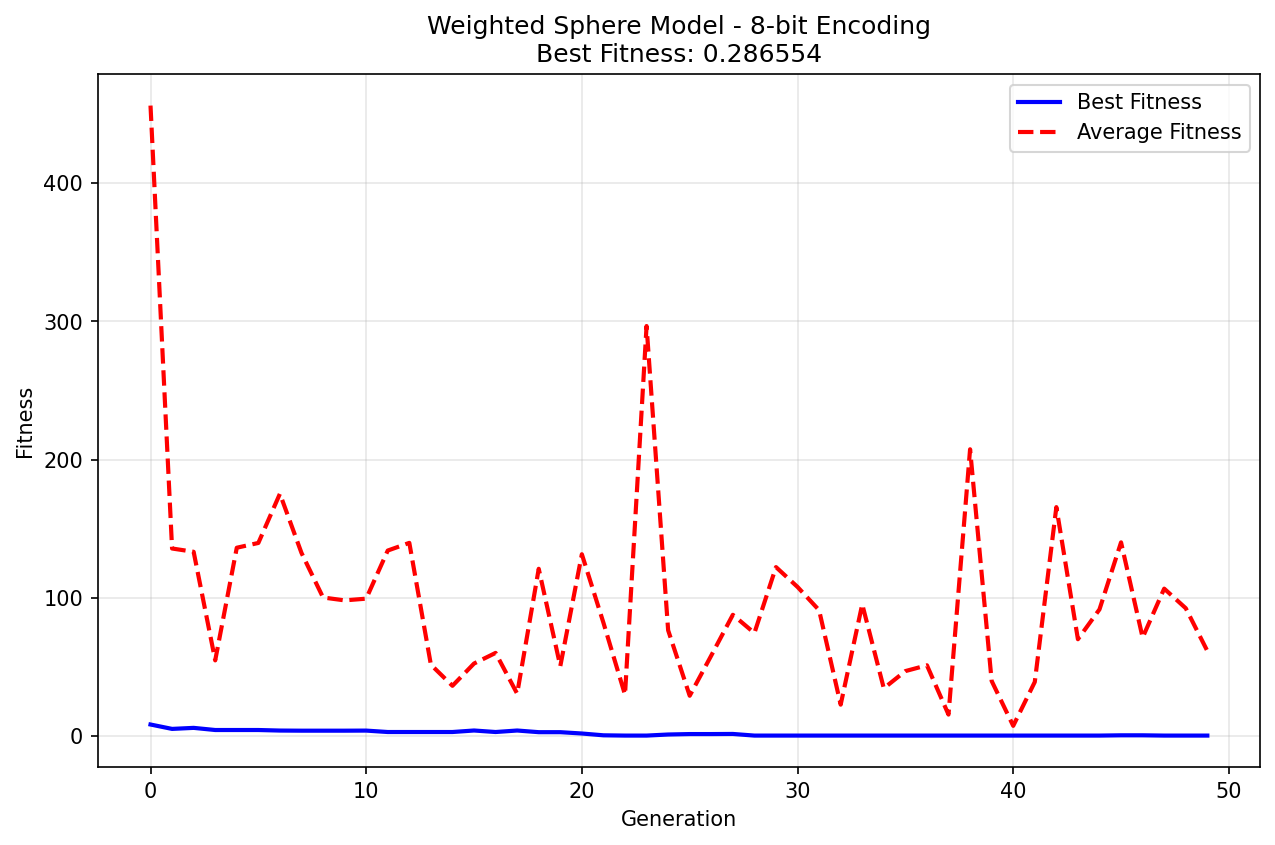
\includegraphics[width=\textwidth]{f2_8bit_fitness.png}
    \caption{8-bit encoding}
\end{subfigure}
\begin{subfigure}{0.48\textwidth}
    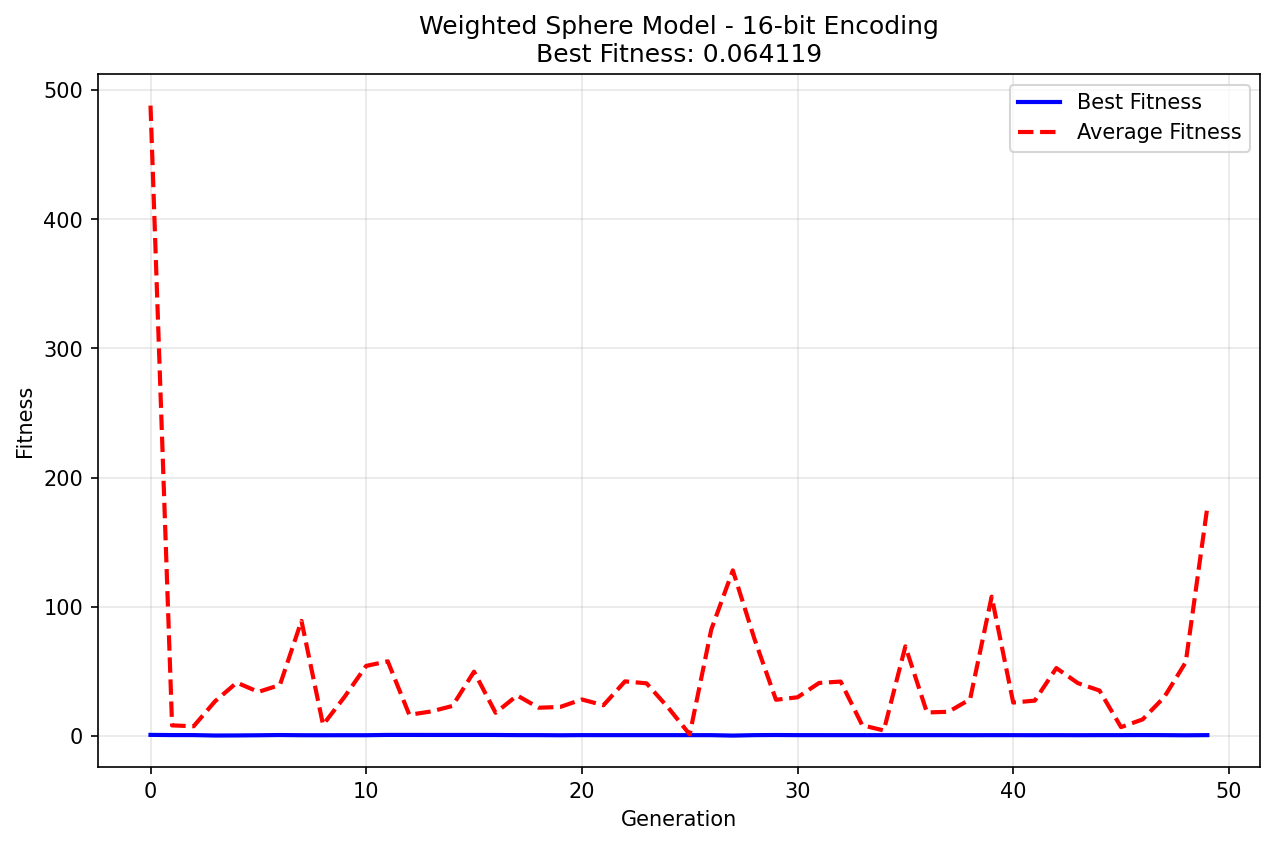
\includegraphics[width=\textwidth]{f2_16bit_fitness.png}
    \caption{16-bit encoding}
\end{subfigure}
\caption{Weighted Sphere Model (f2) convergence behavior}
\label{fig:f2}
\end{figure}

\begin{figure}[H]
\centering
\begin{subfigure}{0.48\textwidth}
    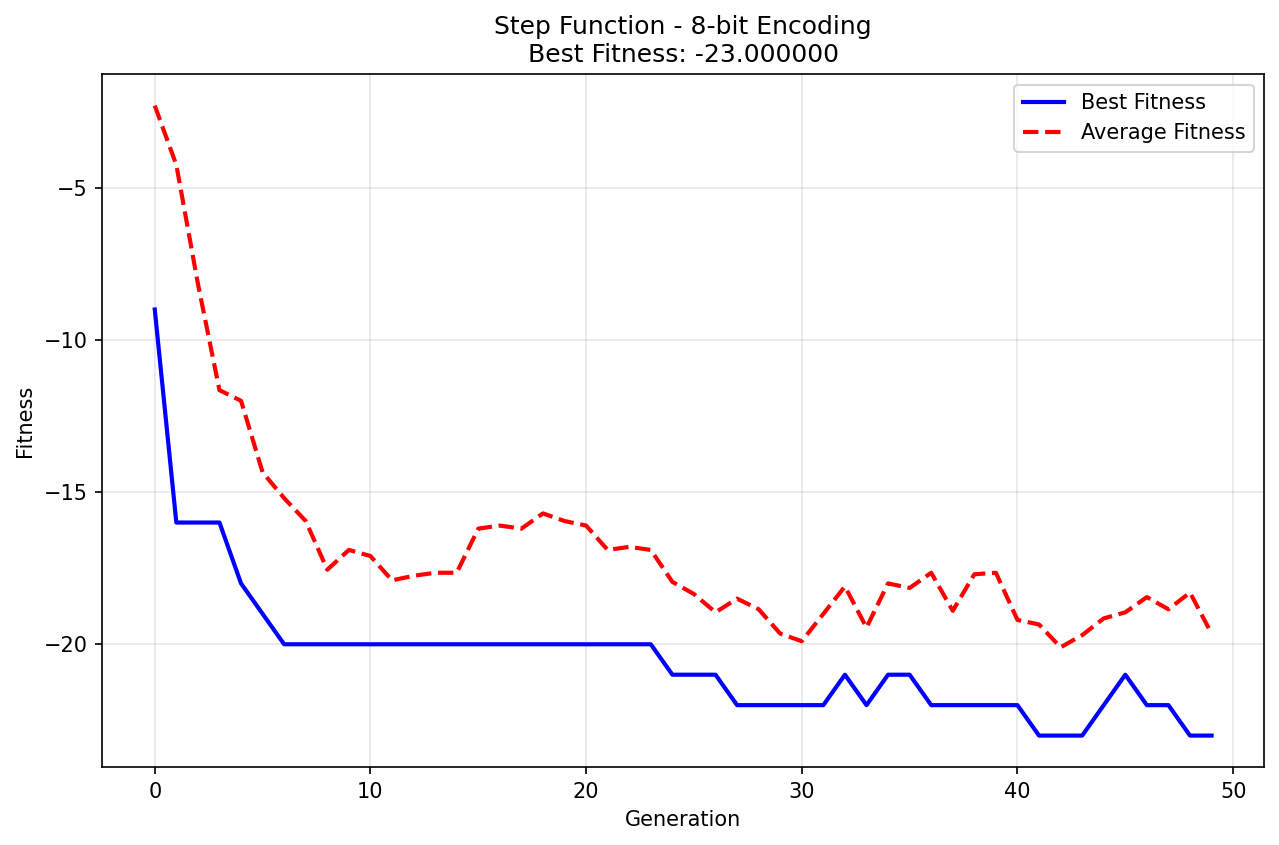
\includegraphics[width=\textwidth]{f3_8bit_fitness.png}
    \caption{8-bit encoding}
\end{subfigure}
\begin{subfigure}{0.48\textwidth}
    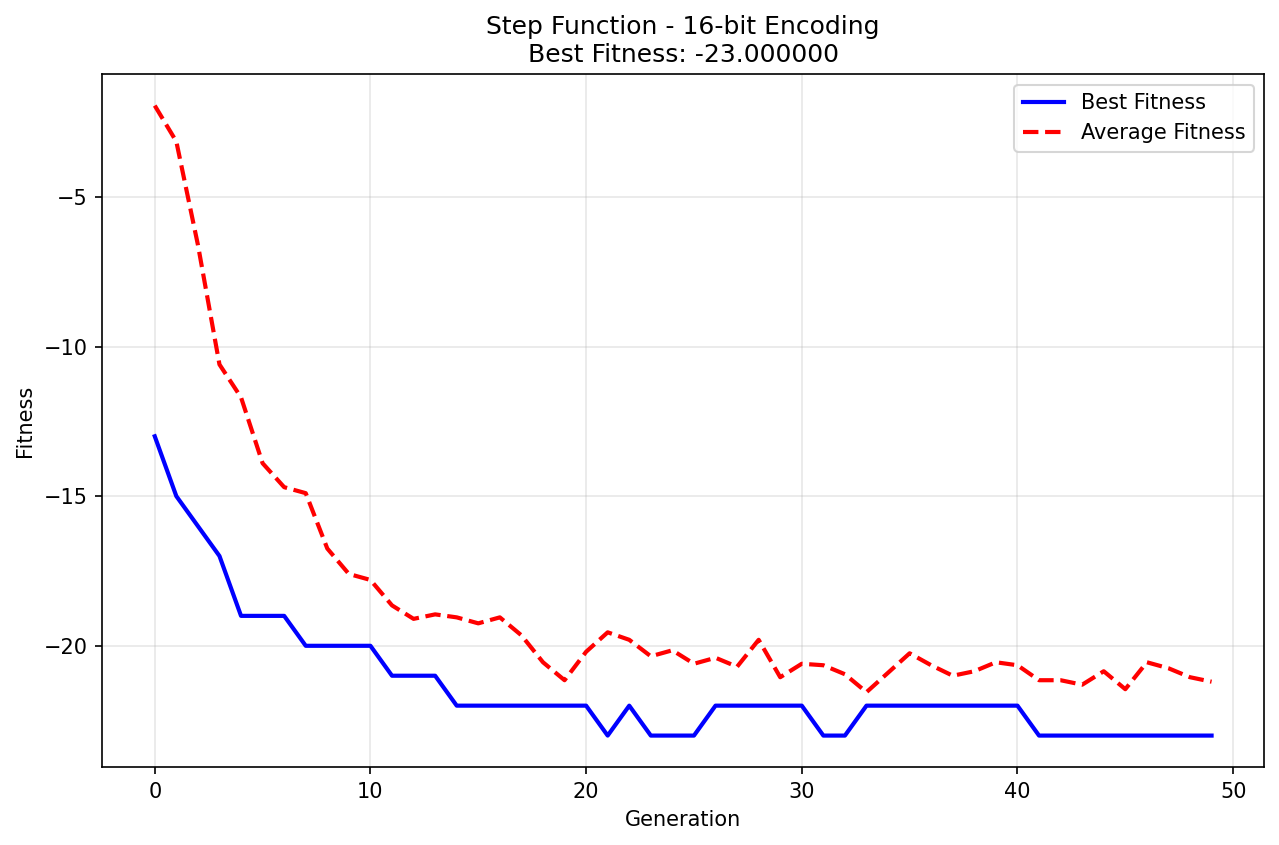
\includegraphics[width=\textwidth]{f3_16bit_fitness.png}
    \caption{16-bit encoding}
\end{subfigure}
\caption{Step Function (f3) convergence behavior}
\label{fig:f3}
\end{figure}

\begin{figure}[H]
\centering
\begin{subfigure}{0.48\textwidth}
    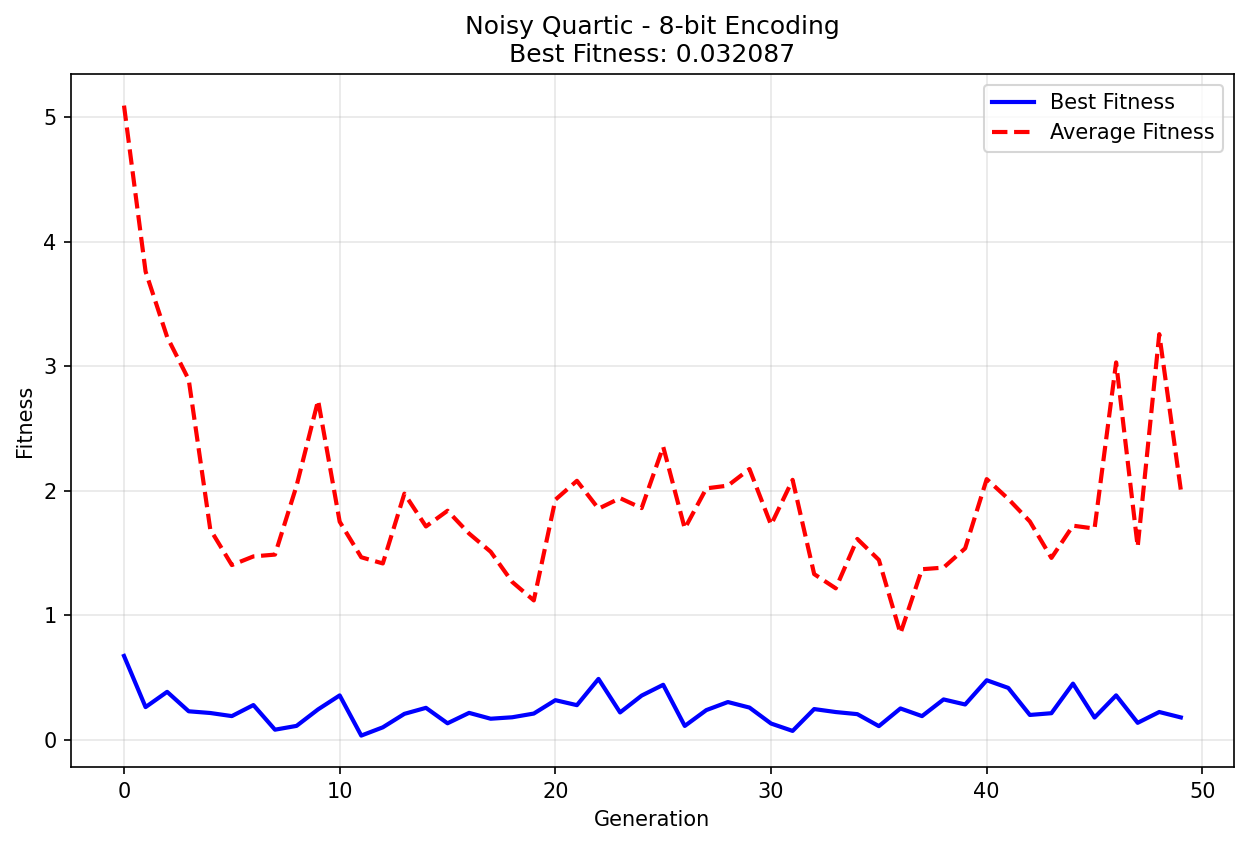
\includegraphics[width=\textwidth]{f4_8bit_fitness.png}
    \caption{8-bit encoding}
\end{subfigure}
\begin{subfigure}{0.48\textwidth}
    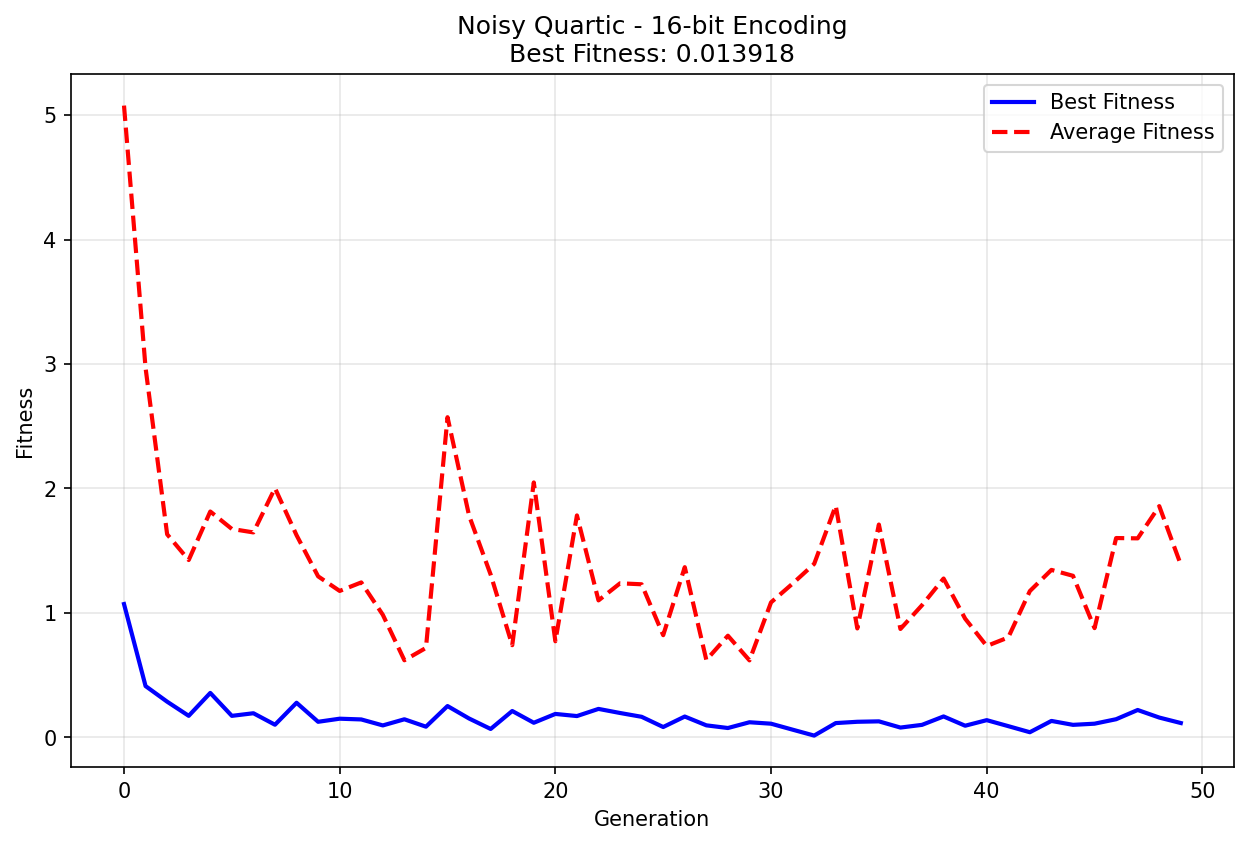
\includegraphics[width=\textwidth]{f4_16bit_fitness.png}
    \caption{16-bit encoding}
\end{subfigure}
\caption{Noisy Quartic (f4) convergence behavior}
\label{fig:f4}
\end{figure}

The plots demonstrate varied convergence patterns. The Sphere function shows rapid convergence within 5-10 generations with smooth fitness curves. The Weighted Sphere exhibits high volatility in average fitness, with spikes reaching 300-500, indicating the challenge of navigating its narrow valley. The Step function displays characteristic discrete jumps in fitness values. The Noisy Quartic shows stable convergence with minor fluctuations due to the stochastic noise component.

\subsection{Best Solution}
Table~\ref{tab:best_solutions} presents the best solutions found for each function and encoding combination.

\begin{table}[H]
\centering
\caption{Best solutions and fitness values achieved by the GA}
\label{tab:best_solutions}
\begin{tabular}{|l|c|c|l|c|}
\hline
\textbf{Function} & \textbf{Bits} & \textbf{Best Fitness} & \textbf{Best Solution} & \textbf{Optimal} \\
\hline
\multirow{2}{*}{f1 (Sphere)} & 8 & 0.0399 & [0.100, 0.141, -0.100] & \multirow{2}{*}{0.0} \\
& 16 & 0.0104 & [0.085, 0.007, -0.056] & \\
\hline
\multirow{2}{*}{f2 (Weighted)} & 8 & 0.2866 & [1.036, 1.020] & \multirow{2}{*}{0.0} \\
& 16 & 0.0641 & [0.792, 0.641] & \\
\hline
\multirow{2}{*}{f3 (Step)} & 8 & -23.0 & [-5.04, -4.96, -5.12, -5.08] & \multirow{2}{*}{-24.0} \\
& 16 & -23.0 & [-5.04, -4.80, -5.04, -5.11] & \\
\hline
\multirow{2}{*}{f4 (Quartic)} & 8 & 0.0321 & [-0.356, 0.015, 0.236, 0.075] & \multirow{2}{*}{$\approx$0.0} \\
& 16 & 0.0139 & [0.292, -0.045, 0.036, 0.091] & \\
\hline
\end{tabular}
\end{table}

The 16-bit encoding consistently achieved better or equal fitness values compared to 8-bit encoding, with improvements most pronounced for continuous functions (f1, f2, f4). The Step function showed no improvement with increased precision due to its discrete nature. All solutions closely approached their respective global optima, demonstrating the GA's effectiveness across diverse function landscapes.

\section{Q5: Analysis and Comparison}

\subsection{Convergence Comparison}
The four De Jong functions exhibited distinctly different convergence behaviors:

\textbf{Sphere Model (f1)} demonstrated the most rapid and stable convergence, with both encodings reaching near-optimal values within 5-10 generations. The smooth, unimodal landscape allowed the GA to quickly identify and exploit the gradient toward the global minimum at the origin.

\textbf{Weighted Sphere Model (f2)} showed the most volatile convergence pattern. While the best fitness improved steadily, average fitness exhibited dramatic spikes (reaching 300-500), indicating frequent population members falling outside the narrow valley. The 16-bit encoding achieved significantly better results (0.064 vs 0.287), demonstrating the importance of precision when navigating constrained search spaces.

\textbf{Step Function (f3)} displayed characteristic discrete improvements, with fitness values changing in integer increments. Both encodings achieved identical results (-23), as the function's discontinuous nature negated any precision advantages. The step-wise convergence pattern reflects the floor operation creating plateaus in the fitness landscape.

\textbf{Noisy Quartic (f4)} converged smoothly despite the stochastic noise term, with the best fitness line showing small fluctuations throughout evolution. The GA effectively averaged out the noise through population-based search, finding near-optimal solutions centered around the origin.

\subsection{Optimization Analysis}
\textbf{Easiest to optimize: Sphere Model (f1)}
\begin{itemize}
    \item Smooth, continuous, and differentiable everywhere
    \item Single global optimum with no local optima
    \item Symmetric bowl shape provides consistent gradient information
    \item Both encodings achieved fitness values within 0.04 of optimal
    \item Minimal variance between runs due to predictable landscape
\end{itemize}

\textbf{Hardest to optimize: Weighted Sphere Model (f2)}
\begin{itemize}
    \item Narrow, curved valley creates a challenging search landscape
    \item Small deviations from the valley result in dramatic fitness penalties
    \item The 100$(x_1^2 - x_2)^2$ term creates steep walls that trap exploration
    \item High sensitivity to precision, as evidenced by 4.5× performance difference between encodings
    \item Volatile average fitness throughout evolution indicates difficulty maintaining good solutions
\end{itemize}

\textbf{Relative difficulty ranking:}
\begin{enumerate}
    \item \textbf{Sphere (f1)}: Easiest - smooth, unimodal landscape
    \item \textbf{Noisy Quartic (f4)}: Moderate - smooth but with noise interference
    \item \textbf{Step Function (f3)}: Moderate-Hard - discrete plateaus hinder gradient information
    \item \textbf{Weighted Sphere (f2)}: Hardest - narrow valley with steep penalties
\end{enumerate}

The analysis reveals that function topology significantly impacts GA performance. Smooth, unimodal functions are readily optimized, while narrow valleys and discontinuities present substantial challenges. The 16-bit encoding provided consistent advantages except where function characteristics (discretization in f3) made precision irrelevant.

\section{Conclusion}
This study successfully implemented a binary-encoded genetic algorithm to optimize four De Jong test functions, demonstrating the algorithm's adaptability across diverse optimization landscapes. The GA achieved near-optimal solutions for all functions, with 16-bit encoding generally outperforming 8-bit encoding due to increased precision. The Sphere function proved easiest to optimize due to its smooth, unimodal nature, while the Weighted Sphere's narrow valley presented the greatest challenge, requiring careful balance between exploration and exploitation. The Step function's discrete landscape and the Noisy Quartic's stochastic evaluation showcased the GA's robustness in handling discontinuities and noise. These results confirm that genetic algorithms provide an effective metaheuristic for global optimization, particularly when traditional gradient-based methods fail due to discontinuities, multimodality, or noise in the objective function.

\end{document}